%************************************************
\chapter{Schedule Processing Tool}\label{ch:cifparser}
 %************************************************
 \section{Introduction}
In order as to move from the existing heterogeneous systems to an ontology based system many existing data sources will need to be made available in a format that allows integration and reasoning. In the rail industry, as with most, much data resides in large relational databases; whilst other data however resides in legacy silos, no two of which are alike. Where pre-existing data resides in relational databases, R2RML tools as discussed in \autoref{ch:litreview}, can be used, however, other data sources will need converting on a case by case basis. A typical industry datasource, requiring conversion is timetable information. This is required by customers for journey planning, however internally it is also needed for timetable planning, train identification, crew rostering, and maintenance planning amongst other tasks. The transition process is a prerequisite for moving to ontology based systems thus it is important to investigate how this will be undertaken. The obstacles to this transition, posed by the dated and industry specific data format as well as the volume of data are representative of the challenges that will be faced moving to ontology based systems. In the case of new data sources they fall into two categories; automatically and manually generated data. In this case automatically generated data includes both the output of other software (such as timetabling software) and sensor data the software either generating or aggregating will output in a linked format. In the case of data to be entered by hand that in turn further sub-divides into data for which good editing and entry tools exist, such as finance or personnel data, and that which is entirely new, or currently only described in free text. For data that is new or only available as free text then the simple lack of editing tools is another barrier to the transition. For large corpora then automated text processing tools would be considered, however, for smaller datasets the time configuring such a tool could be greater than that required to enter the data by hand.

\section{Transition to Linked Data}
The transition has two parts: firstly the domain must be modelled and secondly tools must be designed and implemented to parse the existing data files and make the data the contained available. As discussed in \autoref{ch:litreview} ontology data is considered in two parts: the \say{model}, which is known as the TBox and contains the schema information and the data itself, which is known as the ABox. 

The broader domain was first modelled as part of the work reported by \citet{Tutcher2015}, however, extensions have been made to match the available data. The correct modelling of the domain requires knowledge of both ontology modelled and the domain and as such can represent an obstetrical to transition. This challenge continues to require skilled personnel, however as more of the domain is modelled less will need modelling when new data sources are encountered. 

When modelling is considered, it is imperative not to recreate URIs for items already in the ontology as such the following simple steps are taken:
 \begin{itemize}
	\item Search the Tbox for URIs containing the name of the property or object under consideration;
	\item Search the Tbox for URIs with labels containing the name of the property or object under consideration;
	\item Repeat the above for any common synonyms.
\end{itemize}

Searching has been carried out using the inbuilt search functionality of \say{TopBraid Composer}\footnote{An ontology editing tool, available from: \url{https://www.topquadrant.com/tools/modeling-topbraid-composer-standard-edition/}}, however other tools exist, for example running \say{Agent Ransack}\footnote{a tool similar to \say{grep} which finds text within files, well optimised and presented with a user interface, available from: \url{https://www.mythicsoft.com/agentransack}} over the directory containing a text representation of the ontology gives great certainty that nothing has been missed, at the expense of ease of use.

If an object or property (as appropriate for the concept you wish to model) exists then human judgement needs to be used to decide whether the item found is: a URI that should be reused, a super type, or different concept to that which requires modelling. Since different modelling decisions are sometimes taken at different times, it is important to check both properties and classes for any given concept. Where a concept is not directly related to the domain and may exist in an external ontology it is considered best practice to reference the external ontology rather than redefining the concept.

\subsection{Add items to the model }
If it is necessary to add a concept to the model it is necessary also to place it in the correct layer within the model. The layers are shown in \autoref{fig:RacoonLayers} and discussed in \autoref{sec:prevonto}. When adding items they should be added to the lowest possible layer. If the item will not be required outside the application it should be added to the application layer. If the item will be used outside the application then it should be added to the task layer. If it will be used throughout the rail industry worldwide then, not just within a given sub-domain, then the item should be added to the Rail Core level of the ontology. Additions to the rail core level should only be made with careful consideration as this level is required for any implementation of the Rail Core Ontologies and adding concepts to this level increases the size of the ontology that is required by all implementers. Increasing the size of the ontology affects not only the storage requirements, which are fairly easily met with today's hardware, but also the processing requirements as reasoning is carried out over concepts in this level. Rules, whilst strongly encouraged to model business process as well as data, should reside in a lower level of the ontology, owing to their computational cost. This process is summarised in \autoref{fig:additions}.

 \begin{figure}[!h]
\myfloatalign
{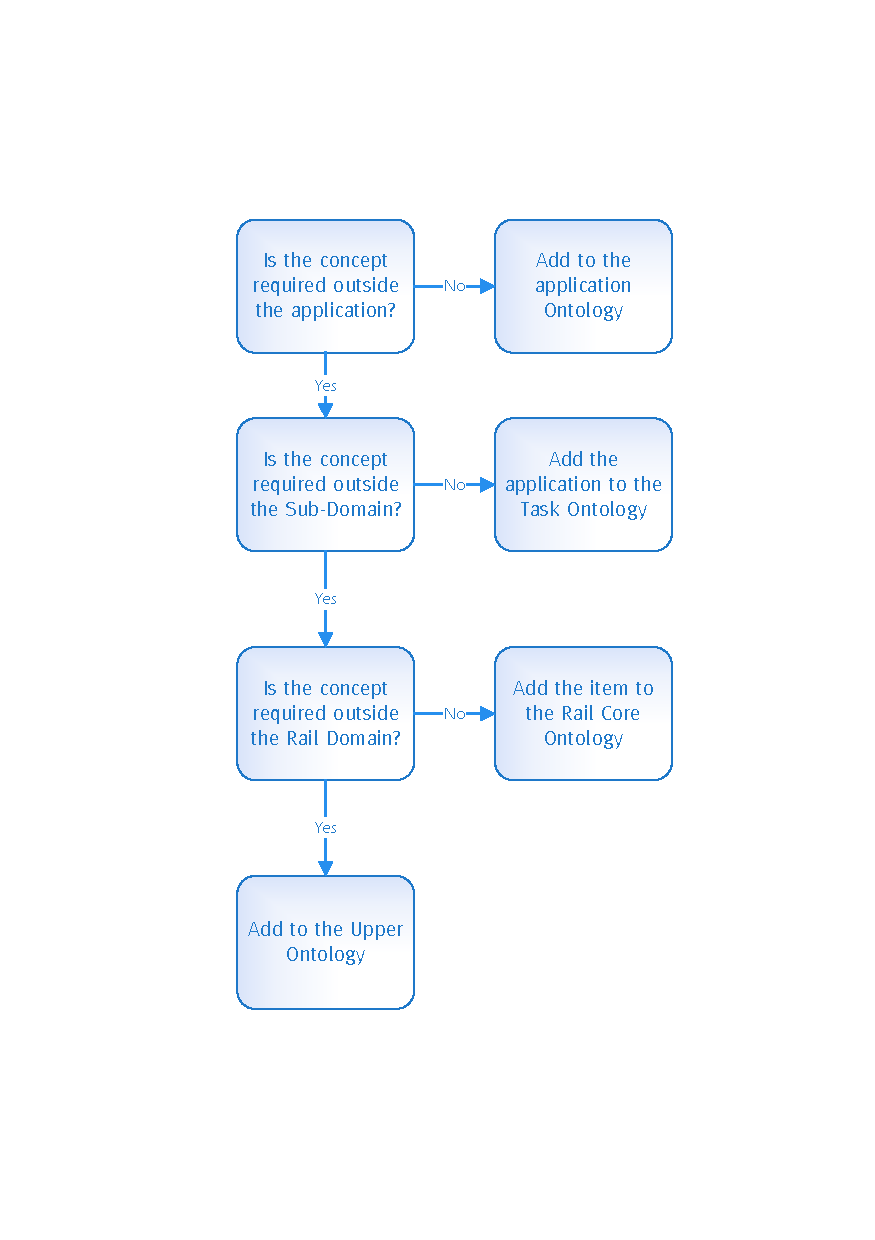
\includegraphics[width=\linewidth]{gfx/AddToOnt}} 
\caption{placing items within the ontology}
\label{fig:additions}
\end{figure}

Once this data is modelled correctly and a tool is designed to insert the abox data in an automated fashion the model will serve as a lingua franca for making the data available to other systems that need it. Additionally it will be possible to use the data in conjunction with other data stored in ontology based systems for reasoning and the abstraction of business process to rules. For example suppose a train operating company wishes to insert an extra service, for a special event at a given time and place, which attracts spectators from many separate points of origin. By combining timetable data with a static map of the network it will be possible to work out whether it is possible to add extra services from various points of origin, given also pricing information and population density data (already available in a linked format, via DBPedia\footnote{Discussed in \autoref{sec:media}}) it would be possible to ascertain the probable profit of each such service. Note that detailed routing information (not in the CIF files) would also be necessary in this scenario. Were the ticket barriers also integrated into such a system it would be possible to sell tickets, at a price determined to make a profit and have them only work on the correct barriers at the correct stations. All of this is possible with the existing disparate systems, but many manual integration steps are required.

\subsection{Tools for parsing A-Box data}

An automated tool is required to parse the A-box data in the following circumstances:

 \begin{itemize}
	\item The data cannot be converted using existing tools, such as OpenRefine\footnote{OpenRefine, formerly Google refine, is a very powerful open source tool which can take data in a wide variety of formats, perform simple processing and output it again in a number of formats, including RDF. More details can be found at: \url{http://openrefine.org/}};
	\item Manual entry is prohibitively slow due to either the volume or velocity of data received.
\end{itemize}

Where the above criteria are met a tool to process the data and add it to the ontology is required. Such a tool would perform the following steps:

 \begin{itemize}
	\item Read the data source;
	\item Convert the data source into a logical in memory representation of that data source, generally objects representing the data structure;
	\item Iterate through the in memory representation inserting each part into the data store.
\end{itemize}


Station location data is also useful in the multi-modal domain. This information is distributed alongside the schedule data and would demonstrate how position data is best modelled. Furthermore by building tools that can process and combine multiple data sources it is possible to show the benefits of using more than one data source together. 
\section{Data to be imported}
\label{sec:datatoimport}
The source of data to represent in a linked format was selected as representative of many that will need to be converted. Additionally since this datasource is used through out the domain it's conversion will bring immediate benefits, as is demonstrated by the use of this tool and datasource as part of the demonstrator discussed in \autoref{ch:COMPASS}. This project considers the use of schedule data to ascertain the destination of a given train on the network.

Currently timetables are exchanged in \say{common interface file} format, as defined in \citep{nr2007}\footnote{Available from: \url{http://www.atoc.org/clientfiles/files/RSPDocuments/20070801.pdf}} first issued in June 1988 and updated regularly since to reflect changes in the UK railway over that time (not least privatisation) this is a representative example of rail data. It is neither easily human readable nor as dense as a pure binary format. Rather it uses fixed length rows of 80 ASCII characters where the interpretation of a row depends on what section it is in.

The schedule file contains the following information:
\begin{itemize}
	\item Schedules
	\item Associations (where trains are split and join for example)
	\item TIPLOC Codes - These are one of the many ways locations are refereed to within the  UK rail network.
\end{itemize}

There is also a header row at the start of the file giving a unique ID to the file and it's issue date and time, along with version information and other meta-data. The file is terminated with a trailer row, to allow users to confirm they have a complete file, though no check sum or similar is employed.

The schedule rows break down further into further subtypes:
\begin{description}
	\item[Basic Schedule] This contains header information pertaining to the entire schedule, such as the type of vehicle and branding of the service.
	\item[Origin Location] The starting point of a service
	\item[Intermediate Location]  A service calling point
	\item[Changes en Route] Where anything contained in the basic schedule field changes over the course of a trains' route.
	\item[Terminating Location] The last call of the service
\end{description}
Not all record types are necessarily present for any given service.

It is possible to ascertain not just the stopping time, and place, of a given service but also some limited meta data, including two different trainIDs, which are also used by other data sources. The first ID given is the so called \say{uniqueID}\footnote{the field is defined by \citet{Hicks} as \say{The unique ID of the schedule being activated - either a letter and five numbers, or a space and five numbers for VSTP trains}. Details available at: \url{http://nrodwiki.rockshore.net/index.php/Train_Activation}} which is also used in by certain other systems (trust train activation messages use this ID), the second ID given is the headcode. Other systems, such as train describers and signalling systems refer to the train by this code. Whilst it is guaranteed a headcode is unique on the rail network at any given point in time more than one timetabled service can have the same headcode.

Each row starts with a 2 letter code to uniquely identify the type of data it holds and some row types are only valid in certain places. For example each train service definition starts with a basic schedule row, then an origin location, followed by any number (including zero) of Intermediate Location's or Changes en Route and finishing with a Terminating Location. 

These files can be used in conjunction with a \say{Master Station Names} file which is typically distributed at the same time. This file provides further detail about the stations refereed to in schedule. Whilst TIPLOC codes are listed in the schedule file alongside a meaningful name in English the geographic position for example is not provided. This is included in the master station names, alongside side details of the type of services that may be connected with (bus or ferry for example) and the Routeing Groups, which are used for fare calculation. By joining on the TIPLOC code it is possible to combine this data with that in the schedule file.

The size of the files to be imported also represents a significant test: the chosen schedule file was 564MB, in what has already been described as a fairly dense data format. This will result in a significantly larger amount of data if exported as turtle, which is a simple text representation of linked data, presenting challenges in terms of both processing time and available RAM. As such the system will need to be carefully optimised to fit within the available memory footprint.

 \section{Software Design}
 Two design patterns were considered to parse schedule files: a state machine and a factory pattern. The state machine pattern, as set out by \cite{Shalyto2006} provides loose coupling between the logic of the program and the state, which is desirable however the transition logic in this case is very straightforward and thus the pattern was disregarded as unnecessary in for this application. The factory technique first discussed in \cite{Gamma2002} is applicable to this system since it abstracts the construction of objects from the point at which they are created, which is beneficial in this case since it is probably that further types of business object will need to be added to design in the future. The system aims to be flexible as to the types of files parsed, importing both \say{Master Station Names} files and Schedules, using the same architecture. In the factory pattern \say{factory classes} are used to construct objects, rather than calling an objects constructor directly. Currently there exist two factory classes, one for each type of file processed, which build the business objects before they are inserted into the datastore. A deliberate benefit of the design is that it is easily possible to add more as required.

 The user interface is made in XAML and partially uses the Model View View-Model design pattern, here on referred to as MVVM, to loosen coupling with the data processing part of the application. The MVVM pattern is described by \citet{Microsoft2012} and is the common way to create user interfaces when using the Windows Presentation Foundation. The windows presentation foundation in turn is a means of creating user interfaces when using the .Net framework on windows desktop machines. The MVVM pattern aims to reduce coupling between the designed user interface, which is purely XAML and describes solely appearance (include elements like mouse over animations) and the way the data is formatted for presentation. In this pattern the data model, provided in this case by the business objects, is independent the view model. In this case the view model is comparatively simple, all that needs to be presented is progress feedback. Data representation and processing is removed again, thus changes to how data is presented (say from a table to a graph) have no impact on the underlying system. A view model is used to format information presented to the user as is required by that pattern, however, normal event handlers still process button click events, rather than using \lstinline{Commands} encouraged in the MVVM design pattern. This is acceptable for this system because if the code is to be reused on another platform or presented differently, for instance as a webservice, then the operations performed in the button click handlers would in any case need to be redesigned. The button click handlers display file selection dialogues for the user, which specific to the platform and not applicable to a webservice. A further benefit of the MVVM design pattern, not capitalised on in a project this small project, is the separation of roles between the user interface design and software development, on larger projects it is possible for the user interface to be developed by a separate team to the code.

 Beyond these specific patterns the program is object originated and makes significant use of inheritance, as is the norm when developing in .Net languages. An example of that inheritance is shown in \autoref{fig:tiplocedItems}, which shows all items use a TIPLOC, a particular type of location code to assert their position. 

 \begin{figure}[!h]
\myfloatalign
{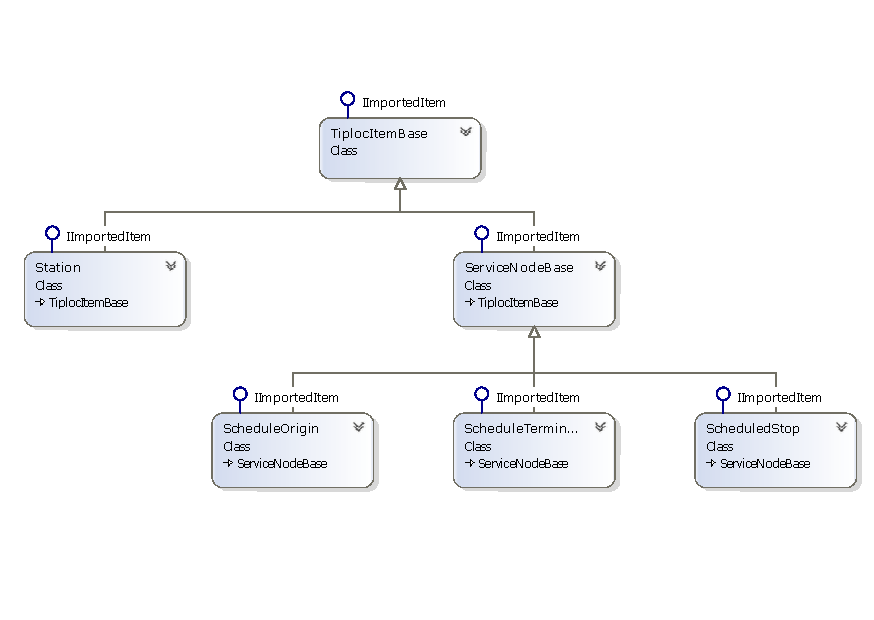
\includegraphics[width=\linewidth]{gfx/ItemsWithTIPLOCsResized}} 
\caption{Items with located using a TIPLOC - one of the location codes}
\label{fig:tiplocedItems}
\end{figure}


 As a result of this design should a new file type need to be parsed the tool could be extended without changes to the existing code. A framework both for reading files into memory and for inserting them into a triple stores is provided.
 \section{Implementation}  
 The system is fairly small and thus all contained in one module and one visual studio project. The code is however organised into four folders which reflect the system organisation. These are:
 \begin{description}
 	\item[Business Objects] These represent the data contained in the source files;
 	\item[DataLink] This handles the connection to any generic linked data store;
 	\item[Stardog Specific] This folder contains functionality for connecting to stardog.
 	\item[GUI] This folder contains folders related to the graphical user interface
 \end{description}

The business objects, as is the norm, represent the data contained in the file, at a low level, both row by row and at slightly higher level representing schedules. All low level business objects implement at interface, namely \lstinline{IImportedItem}, which allows for there population (from a string representing an entire line) and makes it possible to store them to a graph hence an ontology. There exists a factory object for each file type parsed by the system (others can be created as needed) which handles the splitting of the source file into lines, for the creation of business objects and in particular for handling objects which are split across multiple lines, such as schedules. The Business objects and the factories that create them are shown in \autoref{fig:bo}. As is also shown by \autoref{fig:bo} the factory pattern was also used to determine what type of object was required for any given line. A list of factory objects is maintained and each publishes a constant representing the start of the line it should be used with, this could be replaced with a function for more complex situations.

\begin{figure}[!h]
\myfloatalign
{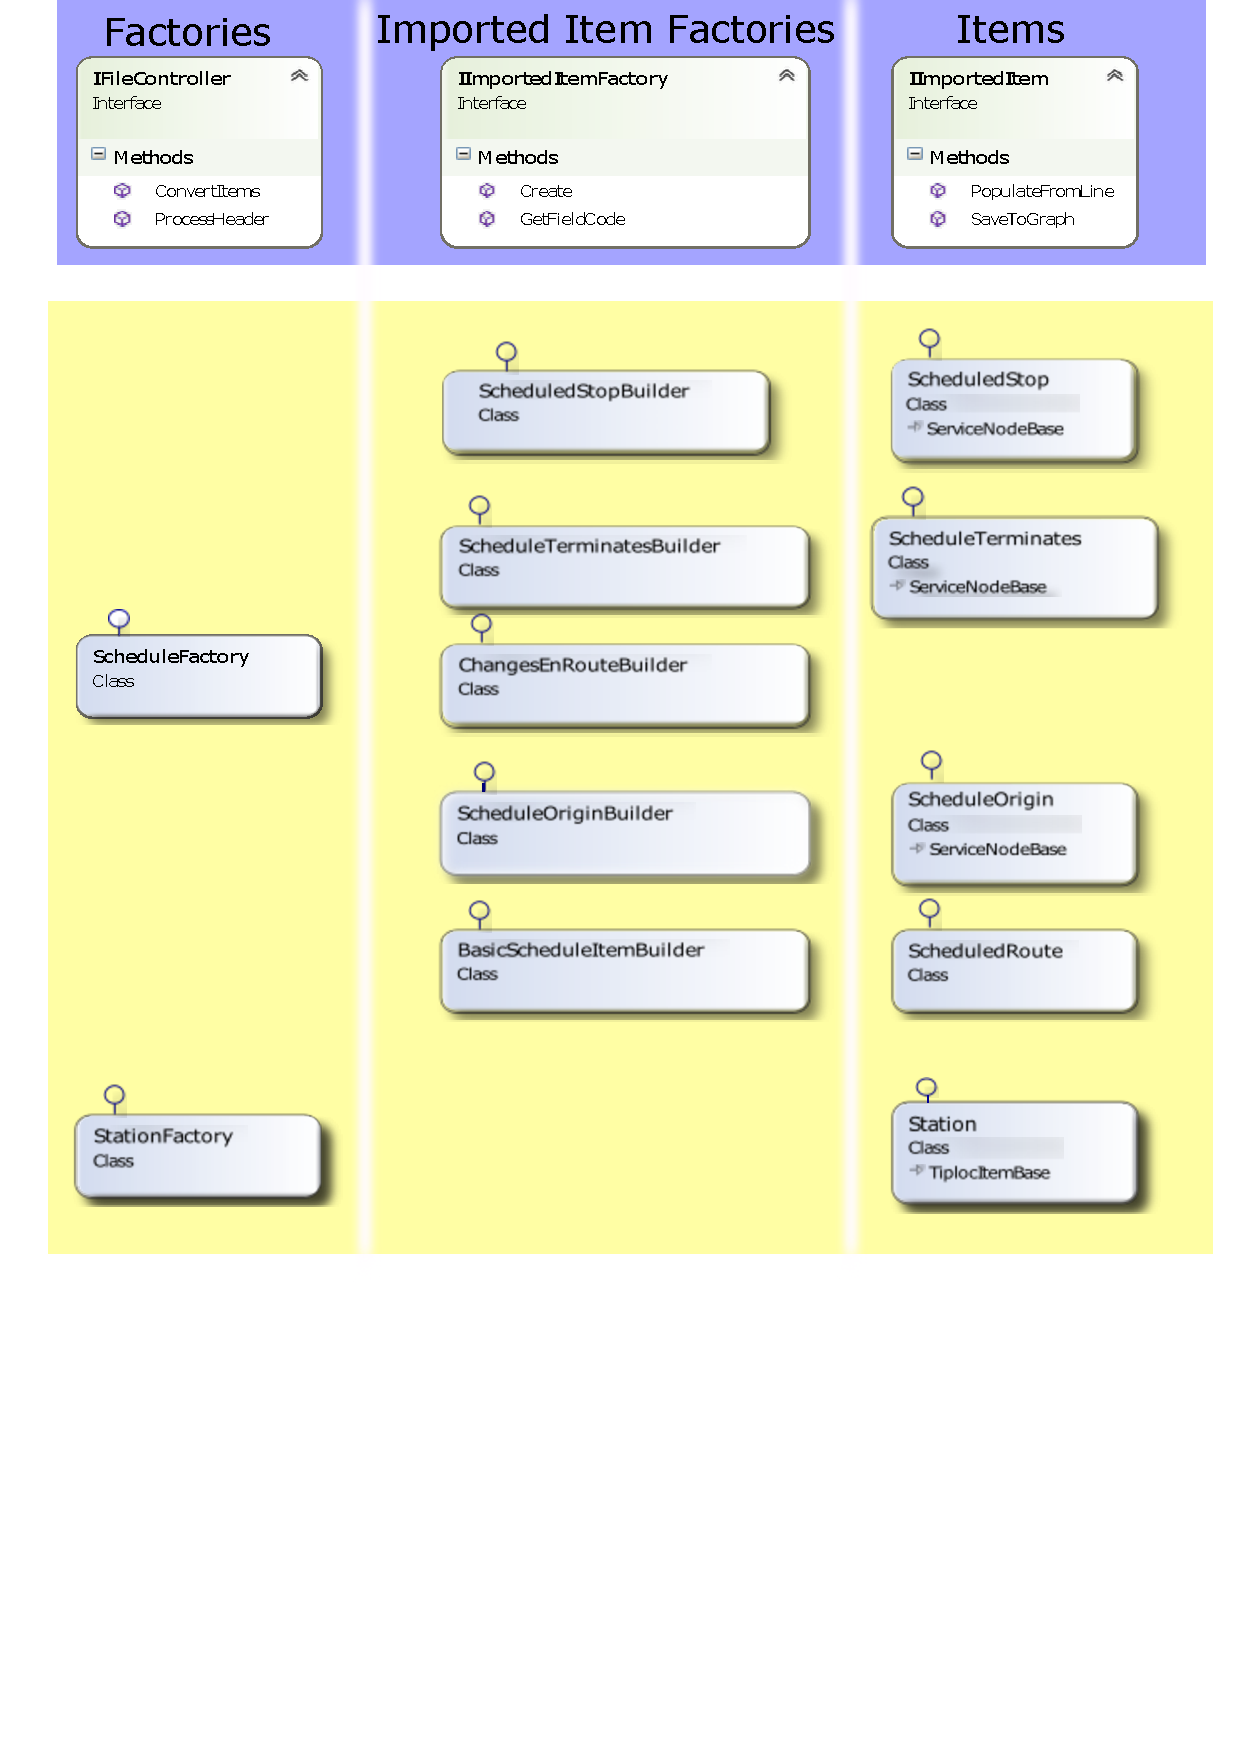
\includegraphics[width=\linewidth]{gfx/BussinessObjectsCat}} 
\caption{Business Object inheritance}
\label{fig:bo}
\end{figure}

When the business objects had been created it became apparent that some of the data they modelled was not modelled by the ontology. These fields were then added as properties in accordance with the guide lines set out in: \citet{Tutcher2015}.

Another .NET practice embraced in this project was the use of the provided settings mechanism for storing constants. This allows for changes to the settings when ever they are required as well as keeping the settings within source control and in one place for easy editing. 

An open source third party library, dotNetRDF was used for connection to local and remote triple stores. This library also allows the construction of graphs in memory and makes it possible to perform reasoning on them. dotNetRDF was selected primarily because it was being actively maintained and was open source, as well as having a complete feature set. 


The most important element of the implementation however was it's heavy use of threading. Given the data volumes involved it was necessary to identify bottlenecks and tasks that could be carried out in parallel and run these on separate threads. The machine used for both development and bench marking has the following pertinent specifications:
\subsection{Hardware Specification}

 	\subsubsection*{Processing} Intel i7-3820\footnote{Intel Data sheet available from: \url{http://ark.intel.com/products/63698/Intel-Core-i7-3820-Processor-10M-Cache-up-to-3_80-GHz}} @ 3.6 GHz. This has 4 cores and can run 8 simultaneous threads.
 	\subsubsection*{Random Access Memory}24 Gigabytes
 	\subsubsection*{Disk} Two Terrabytes, traditional spinning disk, made by Seagate as part of the popular BarraCuda family, model number \texttt{ST2000DM001}. This spins at 7200 rpm and achieves an average data rate (Read and Write) of 156 MB/s.
 
The graphics card fitted (NVIDIA GeForce GTX 650) was of no assistance because none of the tasks in this program were suited to offload to the graphics card.

Bottlenecks were identified by running the \say{Performance Profiler} included with visual studio on the initial version of the software. This can tell the operator which objects are using most of the memory and which functions the program spends longest in. It was apparent from this that most of the memory usage was in the graph constructed by dotNetRDF and most of the processing time was in constructing that graph. Since both the processing time and the memory usage went beyond what was available on the test machine the following steps were taken to enhance performance:
\begin{itemize}
	\item Moved to a 64Bit architecture to remove 4GB limit for memory usage;
	\item Broke the parsed input file and hence the graph built into chunks for processing - each chunk sized to fit in memory. The result of parsing input file, which was a collection of business objects fits easily in memory however when materialised as a graph it was evident from the memory analysis tools it did not;
	\item Parallelised the materialization to a graph. Each graph was separate from others with the intent that they be combined upon insertion into a triple store. This necessitated also parallelised the writing to disk to avoid multiple threads writing to the same file. 
\end{itemize}
 
 The first two steps were required in order as to make the programs memory foot print manageable, where as the last is purely about performance with only the first two steps complete the program was still taking over seventy two hours to execute and thus was impractical in a commercial environment. When re-written as to be multi-threaded it still executed slowly on the test machine, as discussed in results, however given more cores, and in particular faster storage, this design would scale in accordance with the hardware provided.

 In order as to accomplish the multi threaded materialization and writing it was necessary to create a thread pool of data waiting to be processed and written. This uses .Net's underlying thread-pool provision but adds progress feedback and ensures that files are only written after the data is processed.

The data was output as a series of turtle files, which were then inserted into a triple store using a script, rather than inserting directly from the graph owing to limitations of the library. The alternative approach would be to build \texttt{SPARQL} statements that insert the data and run those in chunks of a similar size to the files. This approach would have required more development time as each business object would require functionality to convert it to a part of a \texttt{SPARQL} statement. 

The graphical user interface is simple and shown in \autoref{fig:cifgui}. All that was required was status feedback, for use debugging and to inform the user when the conversion was complete, and buttons to select the files to import. Also available is functionally to add provenance information to the schedules. Provenance information is added to the data when it is inserted in the ontology, allowing the source of the information to be traced, in accordance with the guide lines set out by \citet{Tutcher2015}.

\begin{figure}[!h]
\myfloatalign
\fbox{{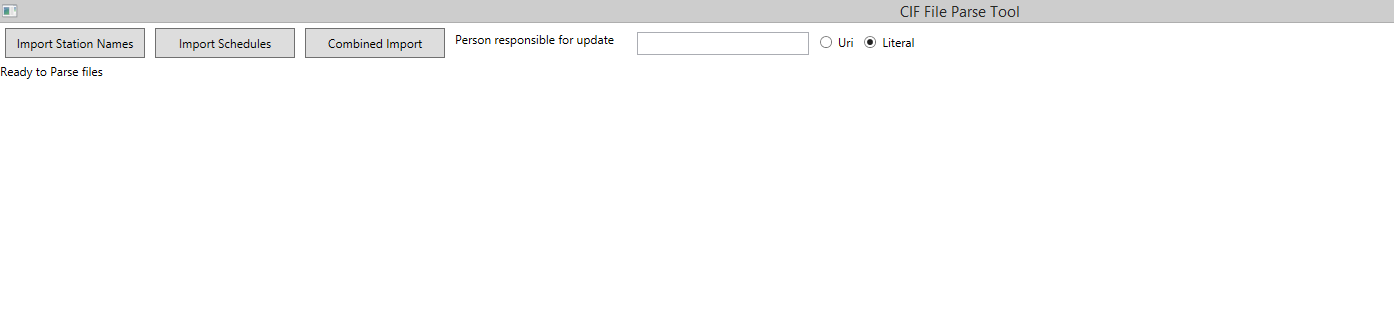
\includegraphics[max height=0.5\textheight,max width=\linewidth]{gfx/cifparseRelevantCorner}} }
\caption{Schedule parsing tool interface}
\label{fig:cifgui}
\end{figure}

\section{Manual Data Entry Tool}
\label{sec:manualtool}
The manual data entry tool demonstrates one possible way that low volume data could be entered. Where such data does not warrant the development of a bespoke tool for the task and it is not possible to interface with or alter the existing tool then a simple universal tool allowing those with no ontology engineering experience to add data to the ontology would be beneficial. There are many pre-existing ontology editors, both open source and commercial, of which protégé and TopBraid Composer were used during this project, however these are better suited to those with some ontology engineering experience. This tool is aimed at those with no ontology engineering experience. This then is another possible answer to the question, \say{\QuestionOtherData}.

\subsection{Implementation}
The tool was constructed as a web application, with intent that it could be deployed centrally in large organisations and used as needed. This tool replies upon the middleware, discussed in \autoref{ch:middleware}, to connect to the triple store. For layout and presentation the popular \say{bootstrap} framework was employed to speed development and allow for access from a range of devices.

As shown by \autoref{fig:mtWelcome} the user is first required to log on. Note that for ease of use all details, except passwords, are stored on the client machine, using cookies.

 \begin{figure}[!h]
\includegraphic[max height=\textheight,max width=\linewidth]{gfx/manToolWelcome}}
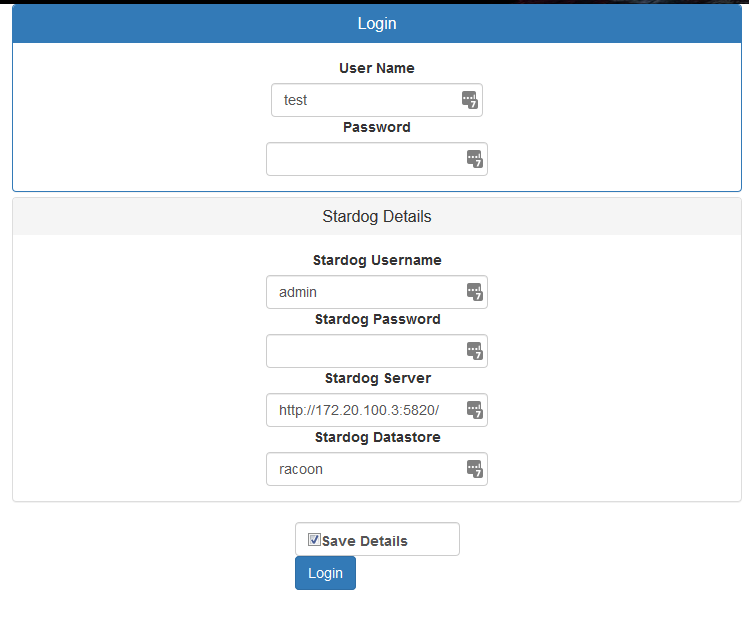
\includegraphics[max height=0.5\textheight,max width=\linewidth]{gfx/manToolLogin}
\caption{Manual Data Entry tool welcome and login screens}
\label{fig:mtLogin}
\end{figure}

As shown in \autoref{fig:mtMainMenu} the system currently supports the following options:
\begin{itemize}
	\item Adding new individuals
	\item Viewing individuals
	\item Uploading data, related to specific project, namely COMPASS as discussed in \autoref{ch:COMPASS}. 
\end{itemize}

 \begin{figure}[!h]
\myfloatalign
{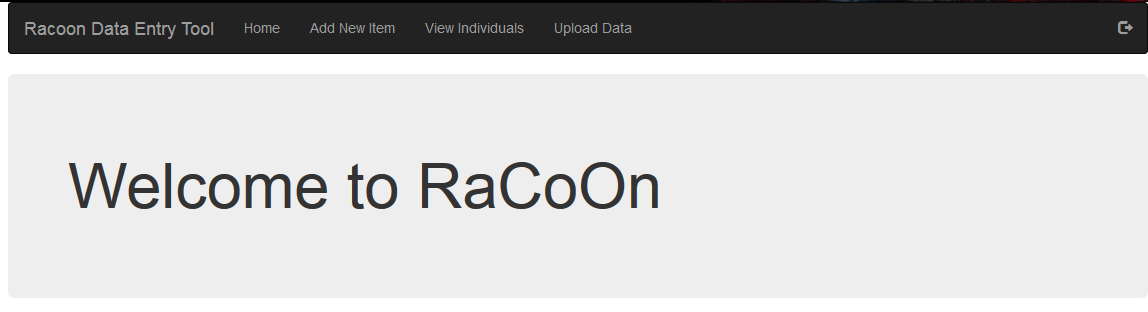
\includegraphics[max height=0.5\textheight,max width=\linewidth]{gfx/manToolInUse}} 
\caption{Manual Data Entry tool main menu}
\label{fig:mtMainMenu}
\end{figure}

The procedure for adding new individuals is set out in \autoref{fig:mtAddingItem} and \autoref{fig:mtAddingItemDetail}

 \begin{figure}[!h]
\myfloatalign
{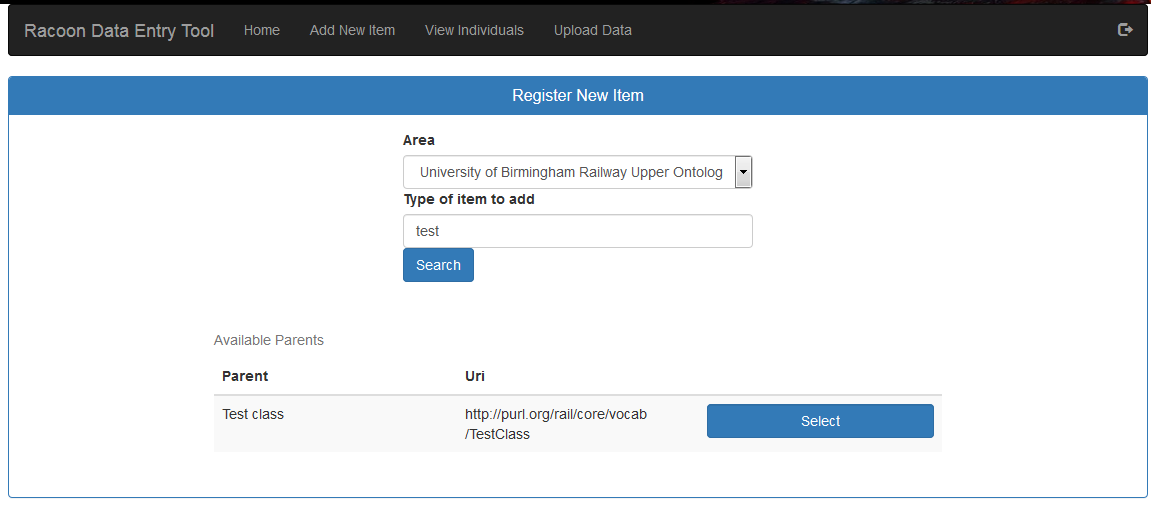
\includegraphics[max height=0.5\textheight,max width=\linewidth]{gfx/manToolAddingItem}} 
\caption{Manual Data Entry tool Adding an item stage one}
\label{fig:mtAddingItem}
\end{figure}

 \begin{figure}[!h]
\myfloatalign
{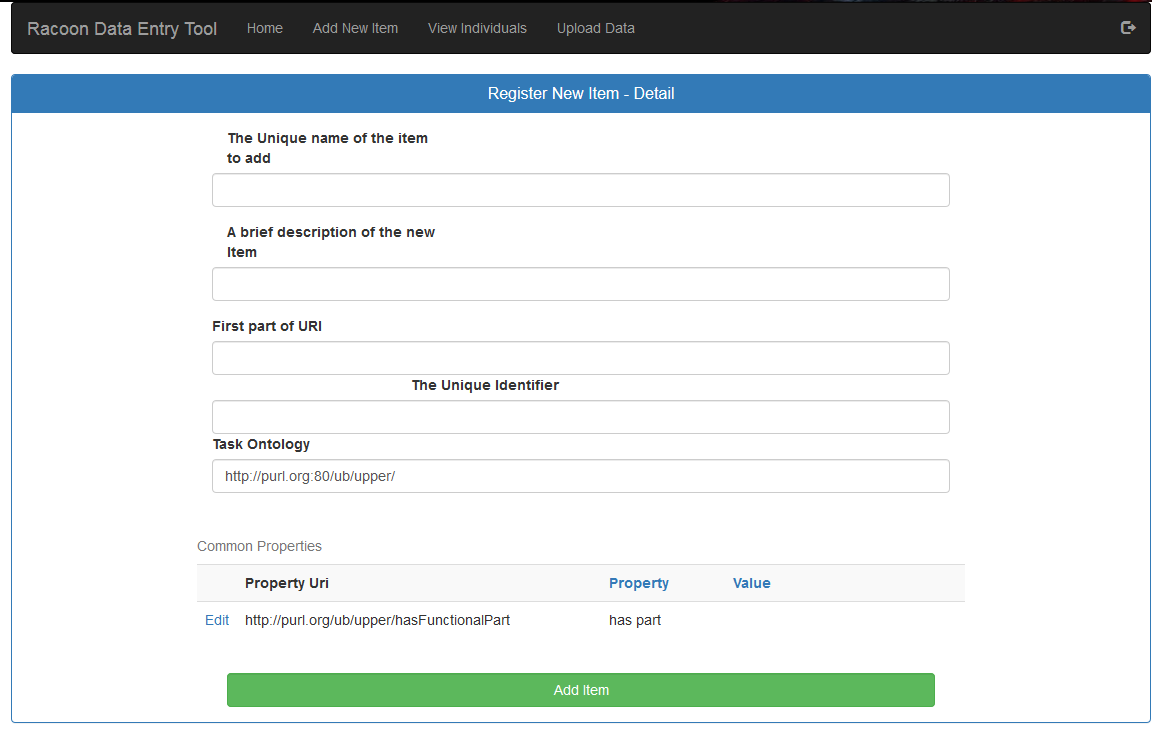
\includegraphics[max height=0.5\textheight,max width=\linewidth]{gfx/addItemDetail}} 
\caption{Manual Data Entry tool Adding an item stage two}
\label{fig:mtAddingItemDetail}
\end{figure}


 \section{Results} 
 Initial tests were performed with smaller schedule files, cut back to 64MB. Even chunks of this size took more than twelve hours using an unoptimised version of the software and when full files were attempted and full files used all available memory before completion. 

The optimised version of the code took two minutes and thirty four seconds to complete a cut down run. The full run took elven hours, fifty five minutes and fourty nine seconds which indicates that further optimisation remains possible. 

The files were quickly and successfully inserted into the triple store (stardog), where it was verified as consistent. 

Log from processing a full weeks schedule.
Processing starts at 17:30:54, processing i.e. converting to graph form takes from 17:30:55 to 17:31:24 then writing the files (which includes building turtle from the graph) takes until 04:25:43. As can clearly been seen from \autoref{fig:cifparsing} in the optimised version performance is linear with time.  In non-optimised versions performance was linear until all memory was consumed at which point it slowed beyond usability. The non optimised version was never run to completion, but had reached approximately 50\% completion after four days. 

 \begin{figure}
\myfloatalign
{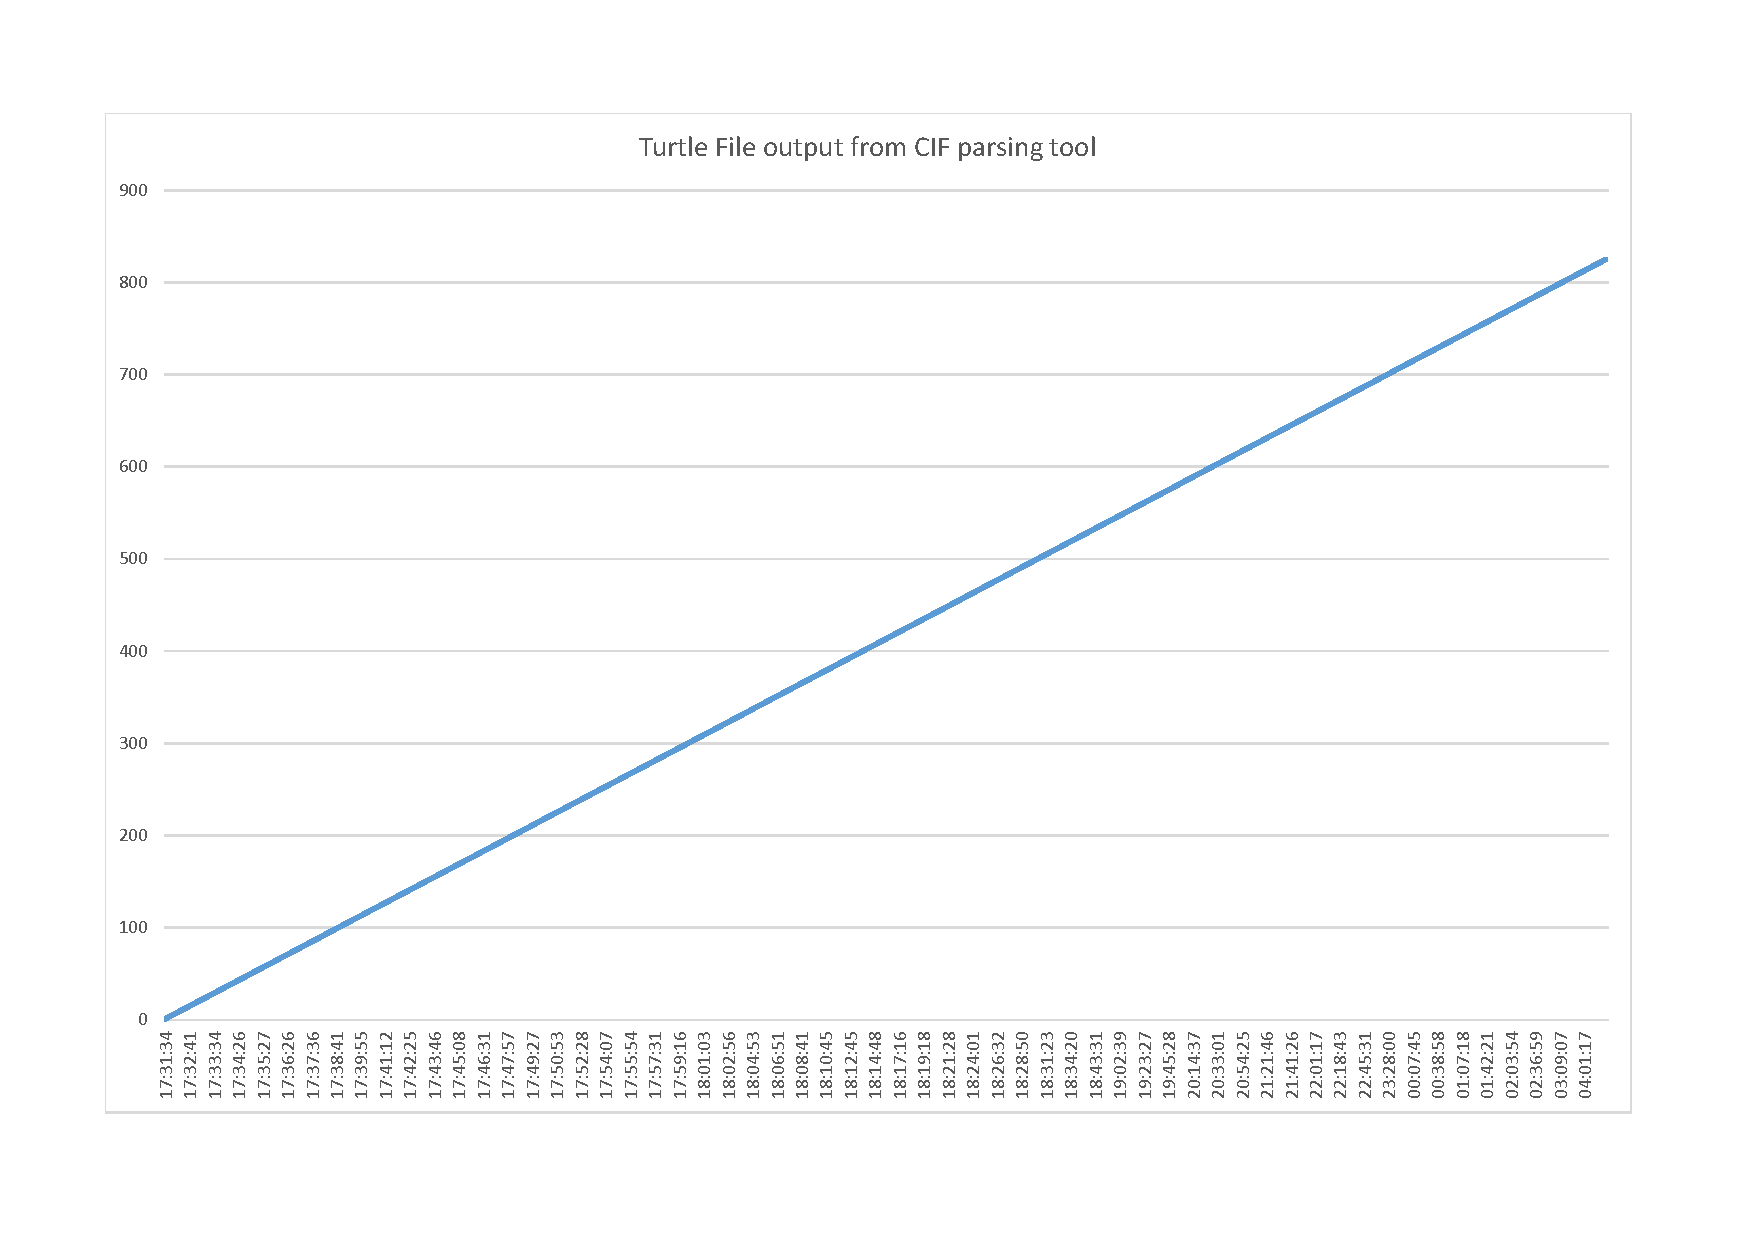
\includegraphics[width=\linewidth]{gfx/scheduleProcessing}} 
\caption{Time to output turtle files}
\label{fig:cifparsing}
\end{figure}

The source code for this tool is available at: \url{https://github.com/Chris-MorrisUK/CifParser}.

\section{Conclusions}

This system was created in response to the following question: \textit{\QuestionOtherData}\\

Firstly this system has proven that it is possible to make typical industry data sources available in a linked format, by taking schedule data, a typical industry data source and making it available as turtle files, which can be loaded into a triple store and queried or reasoned over. 

Secondly this system has shown that even quite small data sources, as compared to video or high data rate sensors for example, require a high degree of optimisation and produce much larger data sets in a linked format. 

This design and implementation of this system also demonstrated that even where the domain has been partially modelled new applications of that model will require small alterations to suit the precise nature of the available data and it's eventual use. This in turn has wide ranging implications for the need for ontology specialists to be involved, lightly at least, in the design phase of future projects making data available as an ontology.

The manual data entry provided another answer to the question \say{\QuestionOtherData}. For some projects the production of bespoke tools won't financially justifiable. Where it is not possible to use commercial off the shelf software to convert data and that data is of a low enougn volume then it will be possible instead to use tools to manually enter that data.

This system has also made it possible to explore: \textit{\QuestionOtherData} \\
The data imported covered the entire UK rail network and whilst it would have required running overnight it was none the less functional. Were the solution to be reworked so as not to create a graph of the data, then store it as turtle, but rather to directly interface with the triple store it may be possible to reduce the running time further.

\section{Further Work}
This tool could be directly connected to a datastore, rather than generating turtle files which then require insertion. This may well allow for faster processing.